% % % % % % % % Festlegung der Dokumentenklasse % % % % % % % % % % %

\documentclass[twoside, a4paper, parskip=half, captions=tableheading]{scrartcl}

\usepackage{scrpage2} % weiter Einstellungen zur Kopf- und Fußzeile %
\usepackage{mathrsfs} % Schreibschrift %
\usepackage{upgreek} % verwendung durch setzen von up vor dem kleinen Grichischen Buchstaben % % kleine Grichische Buchstaben nicht kusiv %
\usepackage{color} % Änderung der Farbe %
\usepackage[usenames,dvipsnames]{xcolor} % Farb name
\usepackage{lastpage} % Bei Seitenanzahl letzte Seite %
\usepackage{amsmath,amssymb,amstext} % Mathe %
\usepackage{geometry} % Seiten breite einrichten %
\usepackage{gauss} % Gauss / Matrix %
\usepackage{stmaryrd} % Weiter Symbole %
\usepackage{dsfont} %  Mathe Symbole (z.B Mengen) %
\usepackage{booktabs} %Tabellen%
\usepackage{isotope} %Isotope darstellen
\usepackage{mathtools}
\usepackage{xfrac} %schräge Brüche in Text
\usepackage{graphicx}
\usepackage{caption}
\usepackage[separate-uncertainty=true]{siunitx}

\geometry{top=25mm, bottom=30mm}

\usepackage{fontspec} % Umlaute + etc %
\usepackage{polyglossia}
\setdefaultlanguage{german}

\usepackage[
  backend=biber,   % use modern biber backend
  autolang=hyphen, % load hyphenation rules for if language of bibentry is not
                   % german, has to be loaded with \setotherlanguages
                   % in the references.bib use langid={en} for english sources
]{biblatex}
\addbibresource{references.bib}  % die Bibliographie einbinden

% % % % % % % Sprache % % % % % % %
\usepackage[autostyle]{csquotes} % Umlaute + etc %
\usepackage{varioref} % Referenz für formeln usw. %

% % % % % % % Bilder, Tabellen % % % % % % %

\usepackage{graphicx}  		% zum Einbinden von Grafiken
\usepackage{xcolor}			% Für die Verwendung von Farben
\usepackage[font=small,		% kleine Schrift für Bildunterschriften
     labelfont=bf,
     position=top			% Fettgedruckte Bildunterschriften
     ]
     {caption}			% Für Bildunterschriften

\usepackage[labelformat=empty]{subcaption}			% Für mehrere Objekte nebeneinander mit eigenen Bildunterschriften


\usepackage{tabularx}			% Erweiterte Befehle für Tabellen
\usepackage{booktabs}			% Für professionele Tabellen, siehe Manual
\usepackage{longtable}			% Für Tabellen, die nicht mehr auf eine Seite passen.
\usepackage{rotating}			% Zum Verdrehen von Objekten. Nur mäßig verwenden.
\usepackage{placeins}			% Begrenzung für Tabellen/Abbildungen mit \FloatBarrier
\usepackage{verbatim}

% % % % % % % Referenzen und Links % % % % % % %

\usepackage{hyperref}	% Verlinkungen innerhalb und außerhalb des PDF-Dokuments
\def\equationautorefname{Gleichung}
\def\figureautorefname{Abbildung}
\def\chapterautorefname{Kapitel}
\def\sectionautorefname{Abschnitt}
\def\subsectionautorefname{Unterabschnitt}
\def\tableautorefname{Tabelle}
\usepackage{url}		% URL öffnen %
\urlstyle{tt}			% Vordefenierter Style URL %

% % % % % % % % Mathe % % % % % % % %

\numberwithin{equation}{subsection}
\numberwithin{equation}{section}
\renewcommand\theequation{\thesubsection.\arabic{equation}}

\renewcommand{\textfraction}{0.2}

%\usepackage{gnuplottex}

% % % % % % % % % % % % % % % % % % % % % % % % % % % %

\newcommand{\Datum}{18.06.2018}
\newcommand{\Datumabgab}{08.06.2018}
\newcommand{\Personenmit}{Paul Becker\\(paul.becker@udo.edu)\), \\ Alina Nasr-Esfahani\\(alina.esfahani@udo.edu\)}
\newcommand{\Personen}{Paul Becker, \\ Alina Nasr-Esfahani}
\newcommand{\Versuch}{Der Operationsverstärker}
\newcommand{\Nummer}{V51}

\definecolor{hellgrau}{gray}{.45}


% % % % % % % % % % % % % % % % % % % % % % % % % % % %

\title{\Versuch}
\author{Paul Becker\\(paul.becker@udo.edu) \and Alina Nasr-Esfahani\\(alina.esfahani@udo.edu)}
\date{Durchführung: \Datum, 1. Abgabe: \Datumabgab}

% % % % % % % % % % % % % % % % % % % % % % % % % % % %

\pagestyle{scrheadings}
\ihead[]{\small{\textcolor{hellgrau}{Versuchs Nummer:\\ \ \ \ \Nummer \\}}}
\chead[]{\small{\textcolor{hellgrau}{\Versuch\\von \Personen}}}
\ohead[]{\small{\textcolor{hellgrau}{Datum: \\ \Datum \\}}}

\ifoot[]{}
\cfoot[]{\thepage}
%\cfoot[]{Seite \thepage \ von \pageref{LastPage}}
\ofoot[]{}

\footskip 15mm
\headsep 15mm
\setlength\parindent{20pt}

\newcommand{\ignore}[1]{}

\begin{document}
\thispagestyle{empty}
\maketitle
\newpage

\setcounter{page}{1}
\tableofcontents
\newpage
\section{Zielsetzung}
Durch Messung des Transmissionskoeffizienten von Rubidiumgas bei Anlegen eines externen Magnetfeldes wird die
Stärke des Erdmagnetfeldes, die Lande-Faktoren und die Spins der Elektronenhülle und des Kerns der Rubidiumisotope
Rb-85 und Rb-87 berechnet.

\section{Theorie}

Für die beiden verwendeten Rubidiumisotope sind Hyperfeinstruktur- und Zeeman-Aufspaltung unterschiedlich. Die damit
verbundenen Kenngrößen - der Landefaktor, das gyromagnetische Verhältnis und der Spin - können mit Hilfe optischen
Pumpens aufgrund der unterschiedlichen Enerdifferenzen sehr präzise gemessen werden.

\subsubsection{Aufspaltung von Energieniveaus}

Quantenzahlen beschreiben Zustand eines Systems. Durch Kernspin und externes Magentfeld kommt es zu Hyperfeinstruktur-
und Zeemann-Aufspaltung.
Der Gesamtdrehimpuls der Elektronenhülle $\vec{J}$ ist über
\begin{equation}
  \vec{\mu}_\text{J} = -g_\text{J}\mu_\text{B}\vec{J} \quad \text{bzw.} \quad |\vec{\mu}_\text{J}| = -g_\text{J}\mu_\text{B}\sqrt{J (J + 1)}
  \label{magnMom}
\end{equation}
mit einem magnetischen Moment verknüpft, dabei ist $\mu_\text{B}$ das Bohrsche Magneton. Das magnetische Moment der gesamten
Elektronenhülle setzt sich aus den magnetischen Momenten von Bahndrehimpuls $\vec{L}$ und Spin $\vec{S}$ zusammen:
\begin{equation}
  \vec{\mu}_\text{J} = \vec{\mu}_\text{L} + \vec{\mu}_\text{S} \quad \text{mit} \quad |\vec{\mu}_\text{J}| = \mu_\text{B}\sqrt{L (L + 1)} \quad \text{und}
  \quad |\vec{\mu}_\text{S}| = g_\text{S}\mu_\text{B}\sqrt{S (S + 1)}.
\end{equation}
$g_\text{S}$ ist der Lande-Faktor des freien Elektrons, der Zusammenhang der magnetischen Momente wird durch den Lande-Faktor
$g_\text{J}$ ausgedrückt.
%$\vec{\mu}_J$ präzediert um $\vec{J}$, sodass für den Betrag gilt:
%\begin{align}
%  \begin{split}
%    |\vec{\mu}_J| &= |\vec{\mu}_L|\cos\beta + |\vec{\mu}_S|\cos\alpha\\
%    \equiv g_J\mu_B\sqrt{J (J + 1)} = & \mu_B\sqrt{L (L + 1)}\cos\beta + g_S\mu_B\sqrt{S (S + 1)}\cos\alpha
%  \end{split}
%\end{align}
Dieser kann aus den Quantenzahlen über
\begin{equation}
  g_\text{J} = \frac{3.0023J(J+1) + 1.0023[S(S+1) - L(L+1)]}{2J(J+1)}
\end{equation}
berechnet werden.

Liegt ein äußeres Magnetfeld an, kommt es zu einer Aufspaltung der Energieniveaus, da das magnetische Moment mit dem Feld
wechselwirkt; die Wechselwirkungsenergie ist
\begin{equation}
  U_\text{magn} = -\vec{\mu}_\text{J}\cdot\vec{B}.
\end{equation}
Da nur die zu $\vec{B}$ parallele Komponente des magnetischen Moments zu diesem Effekt beiträgt, kommt es zu einer Aufspaltung
der Energieniveaus gemäß
\begin{equation}
  U_\text{magn} = M_\text{J}g_\text{J}\mu_\text{B}B,
\end{equation}
wobei $M_\text{J}$ ganzzahlig ist und aus $-J, -J+1, ..., J-1, J$ stammt. Der sogenannte Zeeman-Effekt beschreibt also die
Aufspaltung in $2J+1$ Energieniveaus bei Anlegen eines äußeren Magnetfeldes.

Bei einem nicht-verschwindenden Kernspin kommt es zudem zu einer Aufspaltung in Hyperfeinstrukturniveaus.
Der Gesamtdrehimpuls der Elektronenhülle $\vec{J}$ koppelt an den Drehimpuls des Kerns $\vec{I}$ zum Gesamtdrehimpuls des Atoms
\begin{equation}
  \vec{F} = \vec{J} + \vec{I}.
\end{equation}
Die Energiedifferenz benachbarter Zeeman-Niveaus ist dann
\begin{equation}
  U_\text{UF} = g_\text{F}\mu_\text{B}B.
\end{equation}
Der Lande-Faktor ist in diesem Fall
\begin{equation}
  g_\text{F} \approx g_\text{J}\frac{F(F+1)+J(J+1)-I(I+1)}{2F(F+1)}.
\end{equation}
$F$ läuft von $I+J$ bis $|I-J|$, jedes Hyperfeinniveau spaltet in einem äußeren Magnetfeld in weiter $2F+1$ Zeeman-Niveaus
auf. Für $I=\frac{3}{2}$ ist dies in \autoref{aufspaltung} beispielhaft gezeigt.
\begin{figure}
  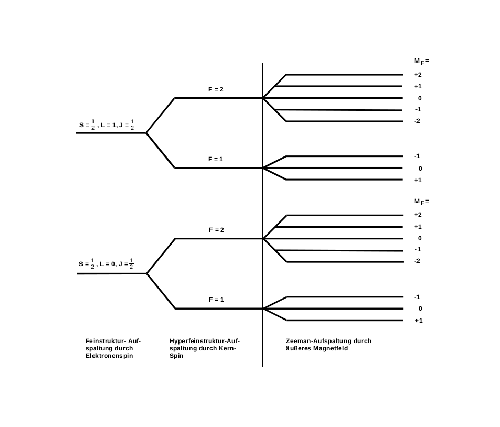
\includegraphics{optischesPumpen/img/aufspaltung.pdf}
  \caption{Hyperfeinstruktur- und Zeeman-Aufspaltung, beispielhaft für ein Alkali-Atom mit $I=\frac{3}{2}$.}
  \label{aufspaltung}
\end{figure}

\subsection{Optisches Pumpen}

Die Energieniveaus der inneren Schalen der Elektronenhülle sind vollstandig besetzt, die Besetzung der äußeren Schalen ist
temperaturabhängig. Im thermischen Gleichgewicht wird sie für zwei Niveaus mit den Energien $W_1$ und $W_2$ durch die
Boltzannsche Gleichung
\begin{align}
  \frac{N_2}{N_1} = \frac{g_2}{g_1}\frac{\exp(-W_2/kT)}{\exp(-W_1/kT)}
  \label{boltz}
\end{align}
beschrieben. $N_i$ sind die Besetzungszahlen der jeweiligen Zustände und die statistischen Gewichte $g_i$ sind ein Maß
dafür, wie viele Zustände es pro Energie $W_i$ gibt.

Der Begriff Optisches Pumpen bezeichnet eine Methode, mit der eine Abweichung von der in \autoref{boltz} gegebenen
Verteilung erzielt werden kann - zum Beispiel in Form einer Inversion, wo $N_2 > N_1$ ist.
Dafür wird Licht eingestrahlt, das gerade die nötige Energie besitzt, um ein Hüllenelektron vom Grundzustand in einen
angeregten Zustand zu versetzen. Für ein Alkali-Atom ist $J=\frac{1}{2}$, $M_\text{J}$ kann also nur $\pm \frac{1}{2}$
werden. Aufgrund der Auswahlregeln sind nur Übergänge mit $\Delta M = 0,\pm 1$ möglich.
Bei $\pi$-Übergangen mit $\Delta M = 0$ wird linear polarisiertes Licht emitiert und absorbiert, für $\sigma^\pm$-Übergänge
mit $\Delta M = \pm 1$ ist es rechtszirkular- bzw. linkszirkular-polarisiertes Licht.
Wird rechtszirkular-polarisiertes Licht in eine Zelle mit dem Dampf eines Alkali-Atom eingestrahlt, können aufgrund der
Beschränkung $\Delta M_\text{J}$ nur Elektronen aus dem energetisch niedrigeren Grundzustand angeregt werden, durch spontane
Emission aus dem angeregten Zustand, werden aber beide Grundzustände bevölkert. Das energieärmere Niveau wird fortlaufend
durch Einstrahlung von Licht geleert, das energetisch höhere, aus dem keine Elektronen angeregt werden können, wird gesättigt.
Als Resultat steigt der Transmissionskoeffizient asymptotisch gegen den Wert 1, da keine Elektronen mehr verfügbar sind, die
angeregt werden können.

\subsection{Messung der Zeeman-Aufspaltung}

Ein Elektron im angeregten Zustand kann durch spontane oder durch angeregte Emission in seinen Grundzustand zurückkehren.
Dabei ist letzteres bei Energien, die für Zeeman-Aufspaltung relevant sind, um 25 Größenordnungen wahrscheinlicher, da die
Übergangswahrscheinlichkeit für spontane Emission $\propto \nu^3$ ist.
Die Zeeman-Aufspaltung tritt nur bei angelgtem Magnetfeld auf, sodass auch nur bei externem Magnetfeld das optische Pumpen
durch Einstrahlen einer geeigneten Lichtquelle in stattfinden kann. Wird ein Magnetfeld angelegt, dass das Erdmagnetfeld gerade ausgleicht, findet keine Aufspaltung statt,
es tritt keine Inversion auf und der Transmissionskoeffizient sinkt.
Ein solcher Einbruch in der Intensität des Lichts tritt auch auf, wenn ein frequenzvariables Hochfrequenzfeld an die
Dampfzelle angelegt wird. Das Magnetfeld wird variiert und sobald es den Wert
\begin{equation}
  B_\text{m} = \frac{4\pi m_0}{\text{e}_0g_\text{J}}\nu
\end{equation}
erreicht, setzt induzierte Emission ein. Die Inversion wird aufgehoben, das eingestrahlte Licht kann wieder absorbiert werden
und der Transmissionskoeffizient fällt ab. Die geschieht jeweils für die beiden Rubidiumisotope bei unterschiedlichem
Magnetfeld.

\subsection{Quadratischer Zeeman-Effekt}

Wird die magnetische Flussdichte vergrößert, müssen bei der Berechnung der Übergangsenergie Terme höherer Ordnung von $B$
berücksichtigt werden, da nun die Spin-Bahn-Wechselwirkung relevant wird. Die Zeeman-Übergänge haben eine unterschiedliche
Energie und sind abhängig von $M_\text{F}$. Der Übergang von einem Zustand $M_\text{F}$ zu $M_\text{F}-1$ mit einer
Hyperfeinstrukturaufspaltung $\Delta E_\text{Hy}$ wird durch die Breit-Rabi-Formel beschrieben:
\begin{equation}
  U_\text{HF} = g_\text{F}\mu_\text{B}B + {g_\text{F}}^2{\mu_\text{B}}^2B^2\frac{1-2M_\text{F}}{\Delta E_\text{Hy}}
\end{equation}

\subsection{Transiente Effekte}

Wird das Hochfrequenzfeld schnell ein- und ausgeschaltet, präzediert der Kernspin um das effektive Magnetfeld. Die
Lamor-Frequenz $\\nu = \gamma B_\text{RF}$ mit dem gyromagnetischen Verhältnis $\gamma = g_\text{f}\frac{\mu_ß}{\text{h}}$
ist vom Lande-Faktor abhängig und somit für die beiden Rubidiumisotope verschieden. Das Verhältnis der Relaxationsperioden
$T = 1/\gamma B_\text{RF}$ ist dann
\begin{equation}
  \frac{T_{87}}{T_{85}} = \frac{\gamma_{85}}{\gamma_{87}}.
\end{equation}

\section{Durchf\"{u}hrung}

Zur Messung der Gitterschwingungen wird ein pump-probe-Aufbau verwendet. Die durch die Oszillation der Gitterschwingungen hervorgerufene, periodische Reflektivitätsänderung wird bestimmt, indem die Intensität des von der Probe reflektierten probe-Laserstrahls mit einer Photodiode gemessen wird. Dazu wird der in \autoref{aufbau} schematisch dargestellte Aufbau zunächst einjustiert. Sowohl der pump-Laser mit einer Wellenlänge von \SI{1047}{\nano\metre} und einem Fokus von \SI{20}{\micro\metre}, als auch der probe-Laser mit einer Wellenlänge von \SI{780}{\nano\metre} und einem Fokus von \SI{2}{\micro\metre} müssen auf die gleiche Stelle auf der Probe gerichtet sein. Das reflektierte Licht muss weiterhin auf die beiden Photodioden treffen.\par
Als erstes wird der Film ohne Höhenprofil angeregt und die Reflektivität gemessen. Daraus wird die Energiedissipation im Galfenol-Film bestimmt. Diese Messung wird im Folgenden von allen weiteren Messungen als Untergrund subtrahiert. Es werden vier Gitter unterschiedlicher Tiefe vermessen und für das tiefste Gitter außerdem die Polarisation gedreht. Aus der Intensität wird die Oszillation der Reflektivitätsänderung der Probe bestimmt. Mit einer Fouriertransformation der Messwerte in der Zeitdomäne lassen sich Amplitude, Frequenz und Breite des Signals untersuchen.
\begin{figure}
  \centering
  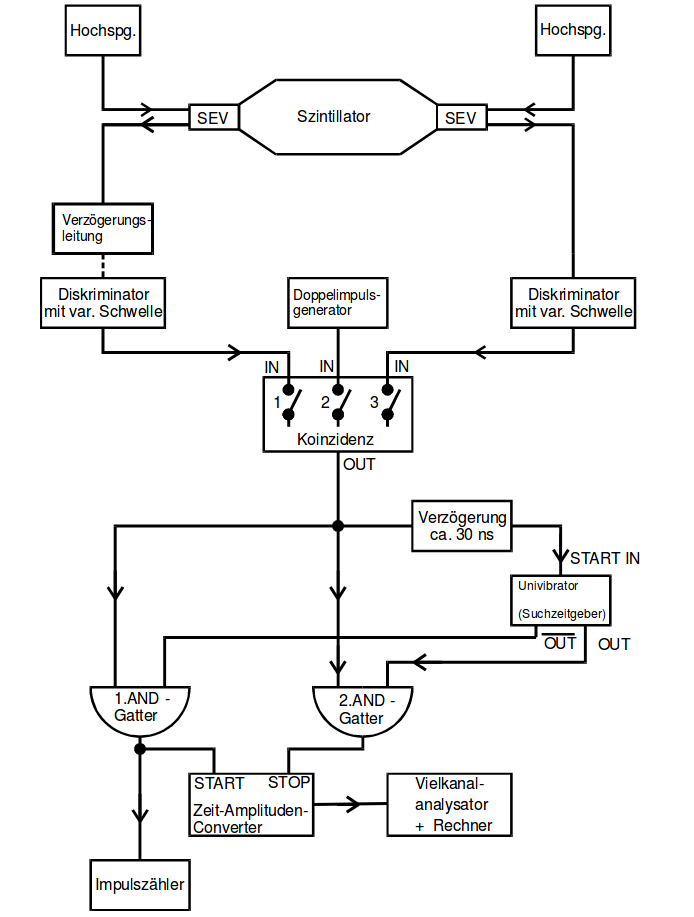
\includegraphics[width=0.75\textwidth]{img/aufbau.png}
  \caption{Schematischer Aufbau der Messapparatur \cite{FP}}
  \label{aufbau}
\end{figure}

\FloatBarrier

\section{Auswertung}

\subsection{Näherung des Films mit Hilfe des drei Temperatur Modell}
Die Messwerte für den Film werden mit Hilfe des drei Temperatur Modells

\begin{equation}
f(x) = A\exp{Bx} + C\exp{Dx} + E\exp{Fx}
\end{equation}

\noindent genähert um anschließend den Anteil des Films aus den weiteres Messungen abziehen zu können.

\begin{figure}[h!]
 	\centering
 	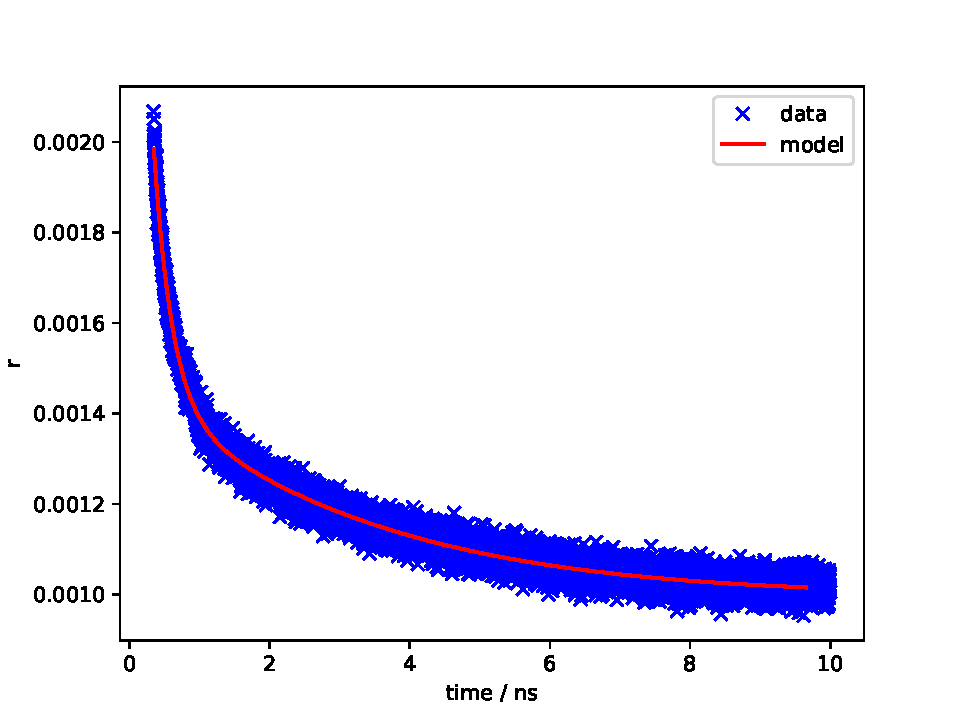
\includegraphics[width=\textwidth]{img/002_a000_b0_e245_FILM.pdf}
 	\caption{Messwerte für den gemesenen Film und die zugehörige Ausgleichsrechnung mit Hilfe des drei Temperatur Modells}
 	\label{abb:film}
\end{figure}

Die Ergebnisse der Ausgleichsrechnung sind in \autoref{abb:film} dargestellt. Die zugehörigen Koeffizienten finden sich in \autoref{tab:fit}.

\begin{table}[h!]
 \centering
\begin{tabular}{cc}
    Koeffizient & Wert \\
	\midrule
 	A & 0.00216 $\pm$ 0.00004 \\
 	B & -3.84 $\pm$ 0.05 \\
 	C & 0.00051 $\pm$ 0.00001 \\
 	D & -0.29 $\pm$ 0.01 \\
 	E & 0.00096 $\pm$ 0.00002 \\
 	F & 0.003 $\pm$ 0.001 \\
\end{tabular}
\caption{Ergenbisse der Ausgleichrechnung mit Hilfe des drei Temperatur Modells}
\label{tab:fit}
\end{table}


\subsection{Korrektur der Daten}
Anschließend wird das Ergebniss der Ausgleichrechnung von den Messwerten der Messungen mit Gitter abgezogen.
In den Folgenden Abbildungen wurde lediglich ein kleiner Teil der Daten gezeichnet um die in den Messdaten enthaltenen 
Oszillationen sichtbar zu machen.

\begin{figure}[h!]
 	\centering
 	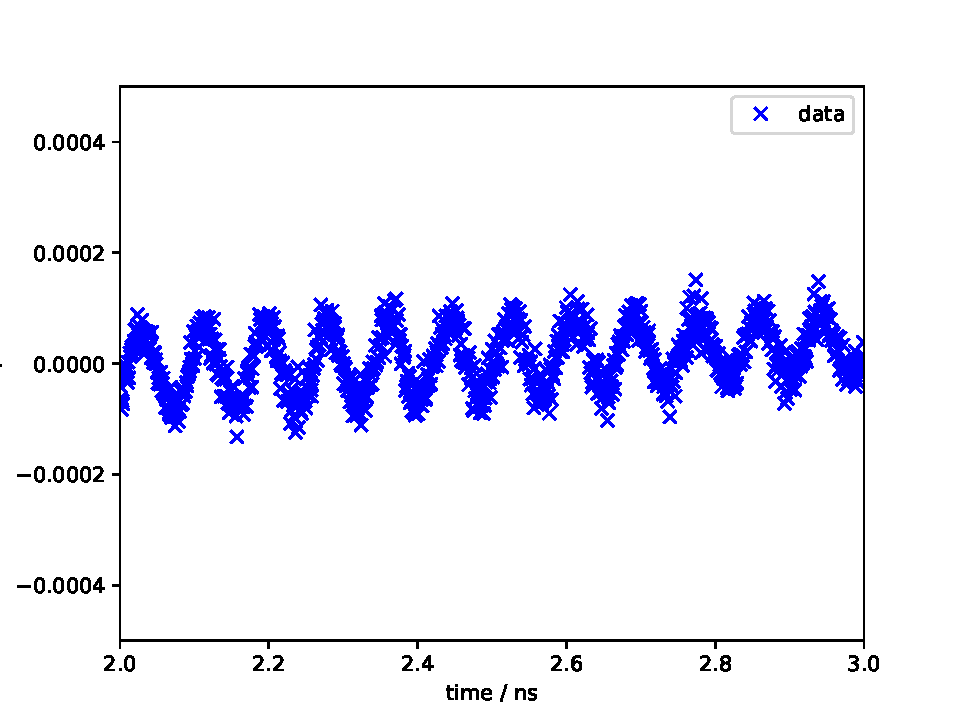
\includegraphics[width=\textwidth]{img/005_a000_b0_e245_G4corr.pdf}
 	\caption{Oszillationen in dem 23 nm tiefen Gitter}
 	\label{abb:film}
\end{figure}

\begin{figure}[h!]
 	\centering
 	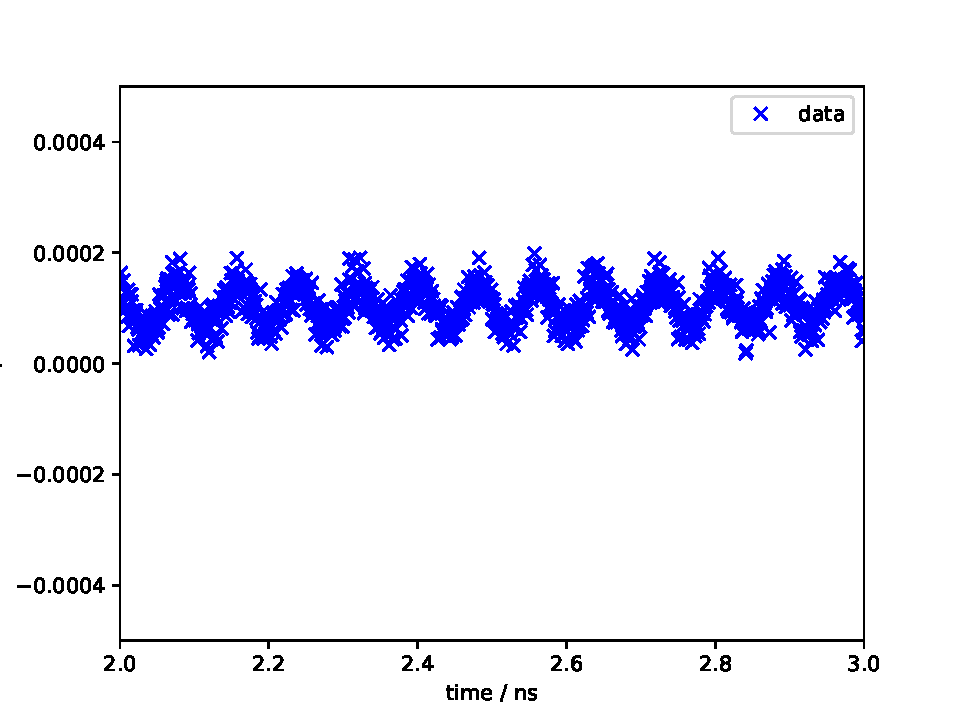
\includegraphics[width=\textwidth]{img/006_a000_b0_e245_G3corr.pdf}
 	\caption{Oszillationen in dem 17 nm tiefen Gitter}
 	\label{abb:film}
\end{figure}

\begin{figure}[h!]
 	\centering
 	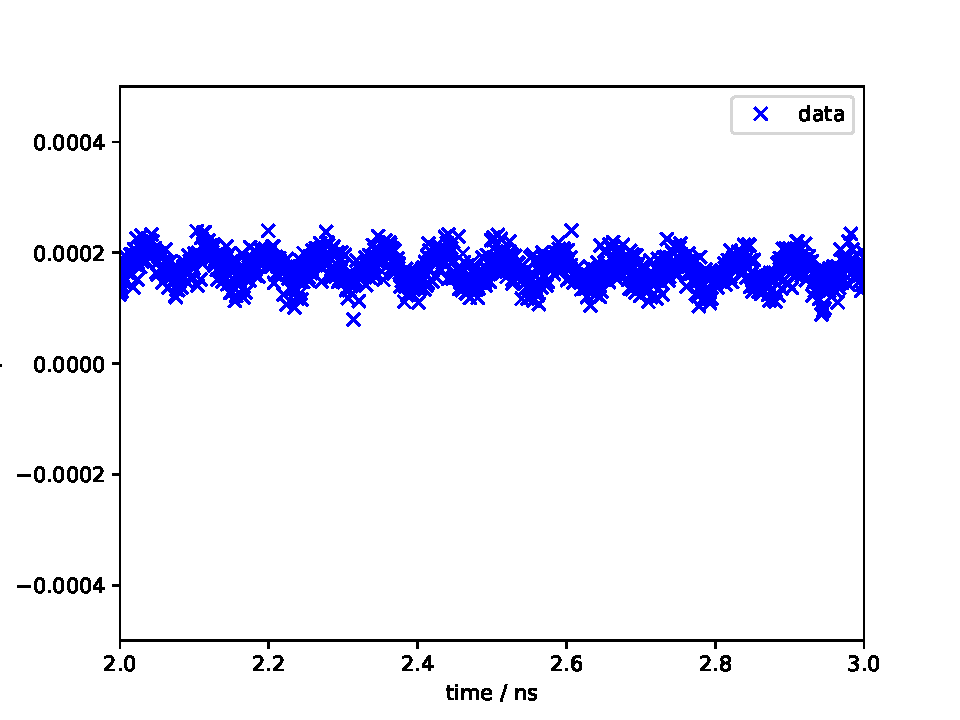
\includegraphics[width=\textwidth]{img/007_a000_b0_e245_G2corr.pdf}
 	\caption{Oszillationen in dem 14 nm tiefen Gitter}
 	\label{abb:film}
\end{figure}

\begin{figure}[h!]
 	\centering
 	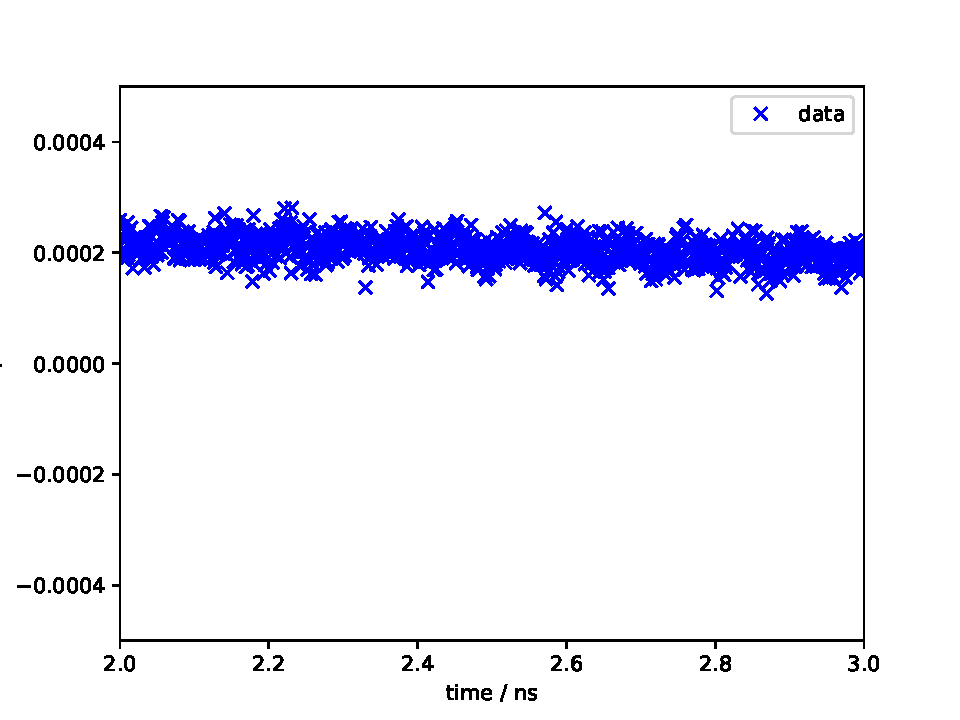
\includegraphics[width=\textwidth]{img/008_a000_b0_e245_G1corr.pdf}
 	\caption{Oszillationen in dem 7 nm tiefen Gitter}
 	\label{abb:film}
\end{figure}


\subsection{Frequenzsprektren}
Die erhaltenen Oszillationen aus den Messdaten werden als periodisches Phänomen aufgefasst und mit Hilfe von Fouriermethoden analysiert. Es fällt auf, dass alle Frequenzspektren einen Peak bei ungefähr 12,5 GHZ aufweisen. Diese Frequenz ist charakteristisch für die benutzen Gitterbreiten und soll im folgenden genauer untersucht werden. An die Peaks wird eine Lorenzkurve gefittet und im Anschluss die Halbwertsbreite und die Amplitude der enthaltenden Frequenz errechnen zu können

\begin{figure}[h!]
 	\centering
 	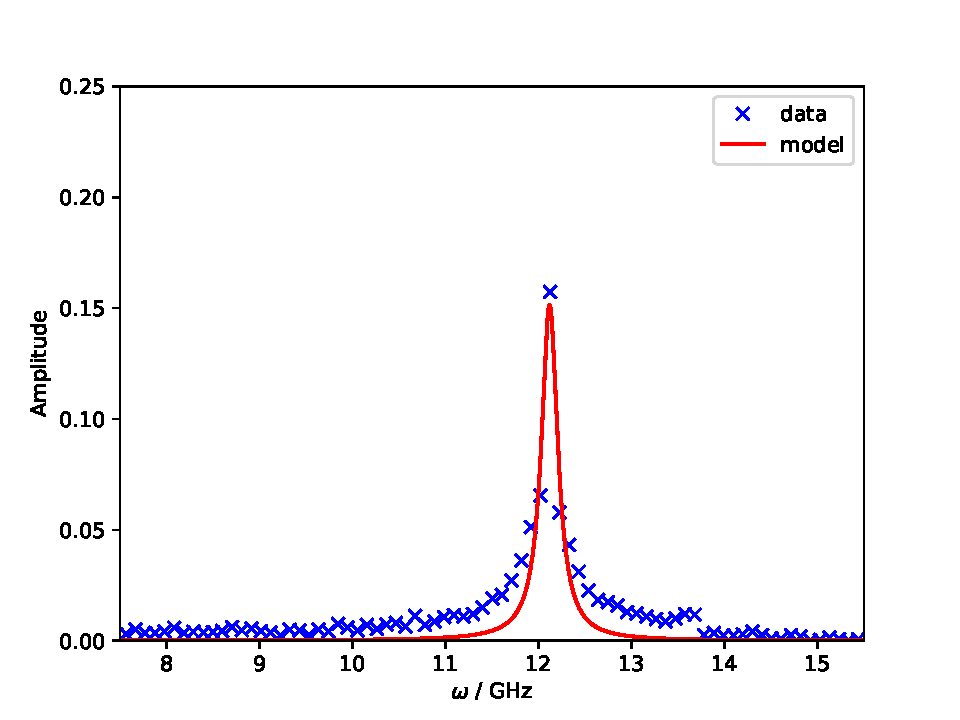
\includegraphics[width=\textwidth]{img/005_a000_b0_e245_G4fft.pdf}
 	\caption{Frequenzsprektrum für das 23\,nm tiefen Gitter}
 	\label{abb:film}
\end{figure}

\begin{table}[h!]
 \centering
\begin{tabular}{cc}
    Koeffizient & Wert \\
	\midrule
 	$\omega_0$ & 12,119 $\pm$ 0,006 \\
 	$\gamma$ & 0,212 $\pm$ 0,004 \\
\end{tabular}
\caption{Fit Ergebnisse für das Gitter mit 23\,nm tiefe}
\label{tab:fit}
\end{table}


\begin{figure}[h!]
 	\centering
 	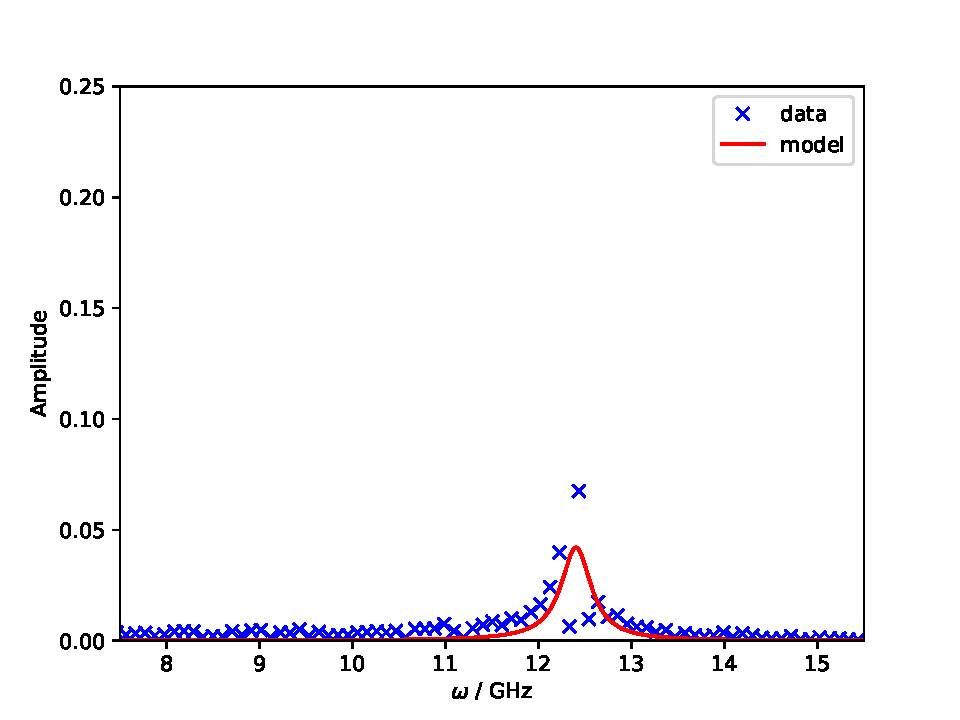
\includegraphics[width=\textwidth]{img/006_a000_b0_e245_G3fft.pdf}
 	\caption{Frequenzsprektrum für das 17\,nm tiefen Gitter}
 	\label{abb:film}
\end{figure}

\begin{table}[h!]
 \centering
\begin{tabular}{cc}
    Koeffizient & Wert \\
	\midrule
 	$\omega_0$ & 12,40 $\pm$ 0,03 \\
 	$\gamma$ & 0,39 $\pm$ 0.03 \\
\end{tabular}
\caption{Fit Ergebnisse für das Gitter mit 17\,nm tiefe}
\label{tab:fit}
\end{table}

\begin{figure}[h!]
 	\centering
 	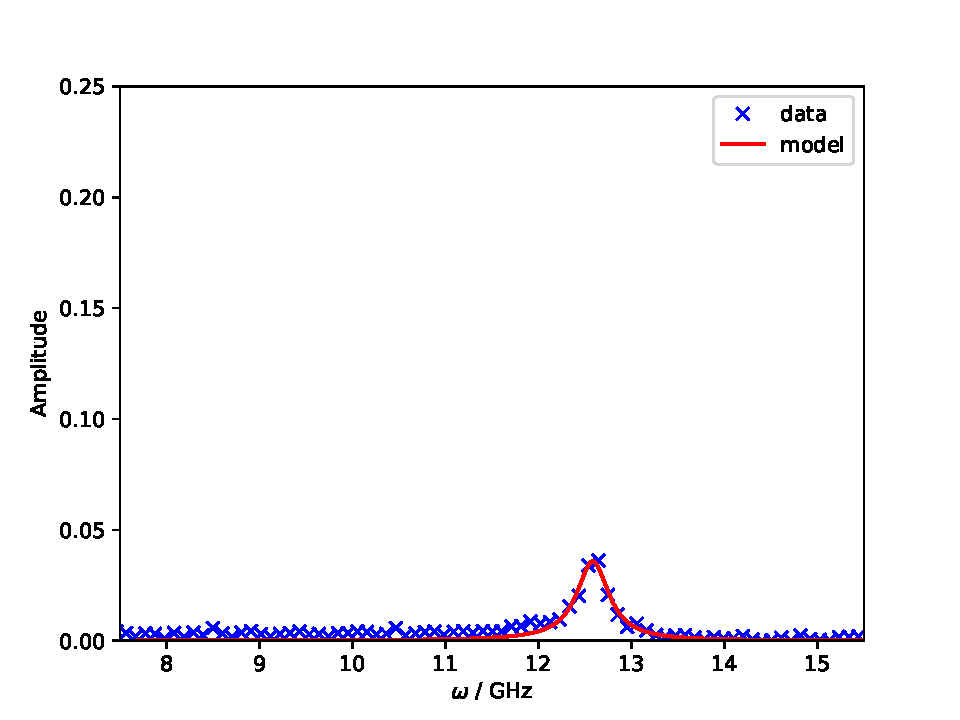
\includegraphics[width=\textwidth]{img/007_a000_b0_e245_G2fft.pdf}
 	\caption{Frequenzsprektrum für das 14\,nm tiefen Gitter}
 	\label{abb:film}
\end{figure}

\begin{table}[h!]
 \centering
\begin{tabular}{cc}
    Koeffizient & Wert \\
	\midrule
 	$\omega_0$ & 12,58 $\pm$ 0.05 \\
 	$\gamma$ & 0,42 $\pm$ 0,04 \\
\end{tabular}
\caption{Fit Ergebnisse für das Gitter mit 14\,nm tiefe}
\label{tab:fit}
\end{table}

\begin{figure}[h!]
 	\centering
 	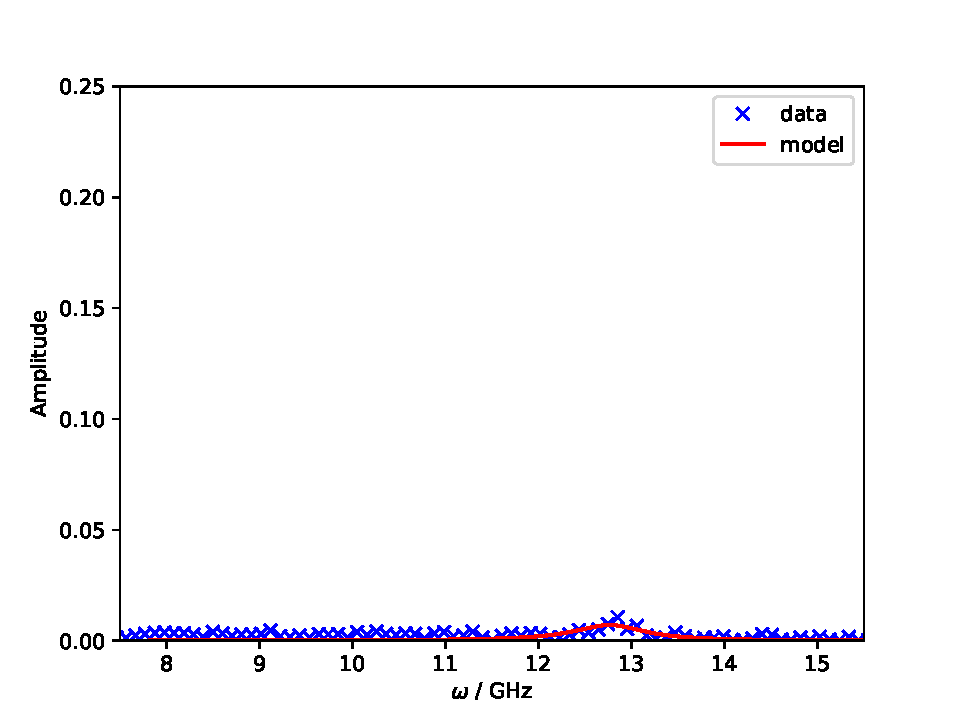
\includegraphics[width=\textwidth]{img/008_a000_b0_e245_G1fft.pdf}
 	\caption{Frequenzsprektrum für das 7\,nm tiefen Gitter}
 	\label{abb:film}
\end{figure}

\begin{table}[h!]
 \centering
\begin{tabular}{cc}
    Koeffizient & Wert \\
	\midrule
 	$\omega_0$ & 12,8 $\pm$ 0,4 \\
 	$\gamma$ & 0,9 $\pm$ 0,4 \\
\end{tabular}
\caption{Fit Ergebnisse für das Gitter mit 7\,nm tiefe}
\label{tab:fit}
\end{table}


Im Anschluss werden die Amplituden der Frequenzkomponenten gegen die Tiefe des Gitters aufgetragen und eine Ausgleichsrechnung
mit einer linearen Funktion

\begin{equation}
f(x) = Ax + B
\end{equation}

durchgeführt.

\begin{figure}[h!]
 	\centering
 	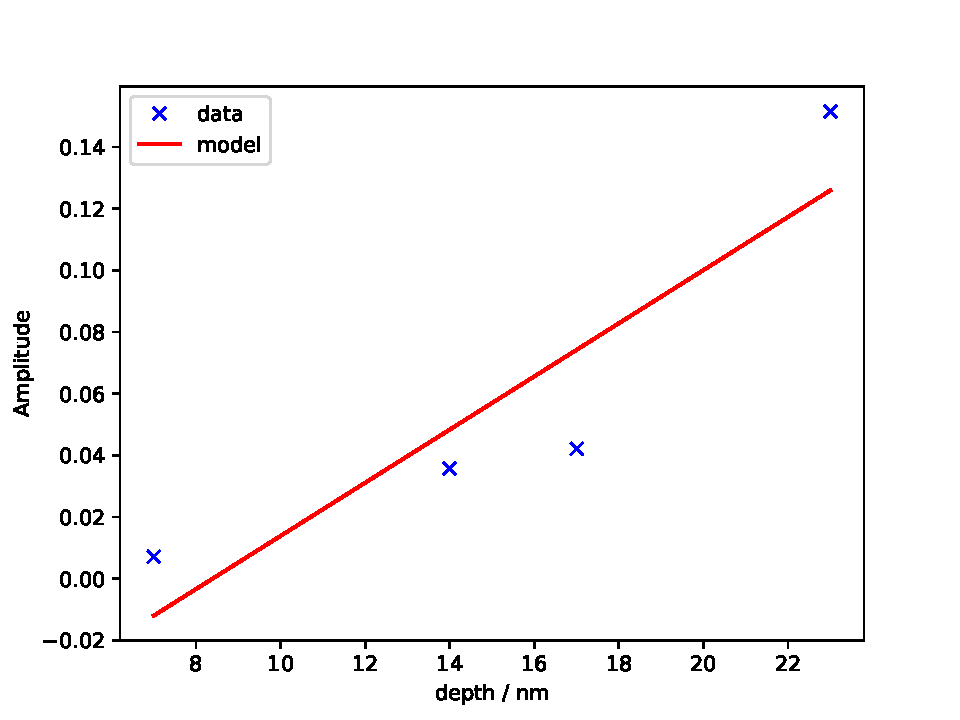
\includegraphics[width=\textwidth]{img/amplitudes.pdf}
 	\caption{Amplituden der charakteristischen Frequenzkomponente aufgetragen gegen die Gittertiefe und linearer Ausgleichsrechnung}
 	\label{abb:film}
\end{figure}

\begin{table}[h!]
 \centering
\begin{tabular}{cc}
    Koeffizient & Wert \\
	\midrule
 	A & 0.009 $\pm$ 0,003 \\
 	B & -0.07 $\pm$ 0,05 \\
\end{tabular}
\caption{Fit Ergebnisse für die Amplituden der verschiedenen Gitter in Abhängigkeit zur Gittertiefe}
\label{tab:fit}
\end{table}

\section{Einfluss der Polarisation auf die Schwingung}

\begin{figure}[h!]
 	\centering
 	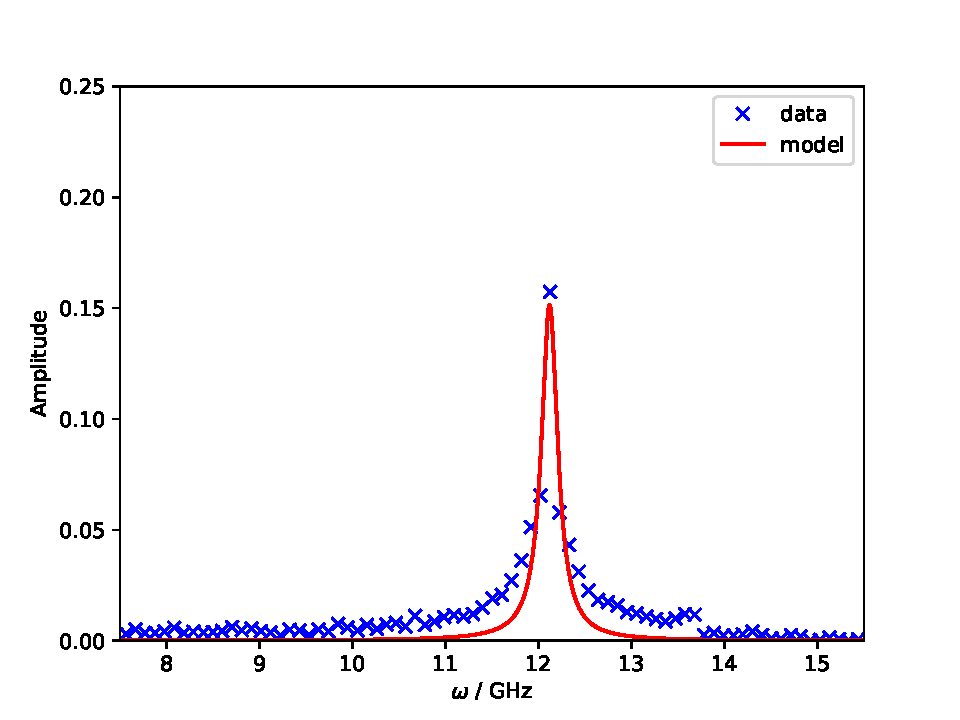
\includegraphics[width=\textwidth]{img/005_a000_b0_e245_G4fft.pdf}
 	\caption{Frequenzsprektrum für das 14\,nm tiefen Gitter unter einem Polarisationwinkel von 0 Grad}
 	\label{abb:film}
\end{figure}

\begin{table}[h!]
 \centering
\begin{tabular}{cc}
    Koeffizient & Wert \\
	\midrule
 	$\omega_0$ & 12,8 $\pm$ 0,4 \\
 	$\gamma$ & 0,9 $\pm$ 0,4 \\
\end{tabular}
\caption{Fit Ergebnisse für das Gitter mit 23\,nm tiefe unter einem Polarisationswinkel von 0 Grad}
\label{tab:fit}
\end{table}

\begin{figure}[h!]
 	\centering
 	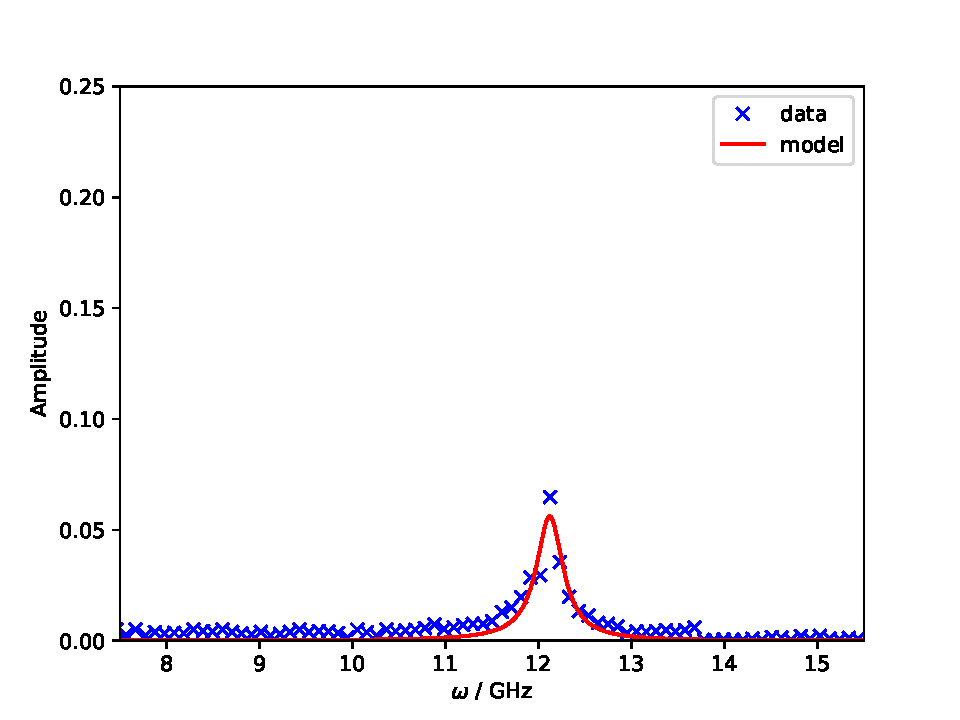
\includegraphics[width=\textwidth]{img/011_a000_b0_e245_G4_45fft.pdf}
 	\caption{Frequenzsprektrum für das 23\,nm tiefen Gitter unter einem Polarisationswinkel von 45 Grad}
 	\label{abb:film}
\end{figure}

\begin{table}[h!]
 \centering
\begin{tabular}{cc}
    Koeffizient & Wert \\
	\midrule
 	$\omega_0$ & 12,8 $\pm$ 0,4 \\
 	$\gamma$ & 0,9 $\pm$ 0,4 \\
\end{tabular}
\caption{Fit Ergebnisse für das Gitter mit 23\,nm tiefe unter einem Polarisationswinkel von 45 Grad}
\label{tab:fit}
\end{table}

\begin{figure}[h!]
 	\centering
 	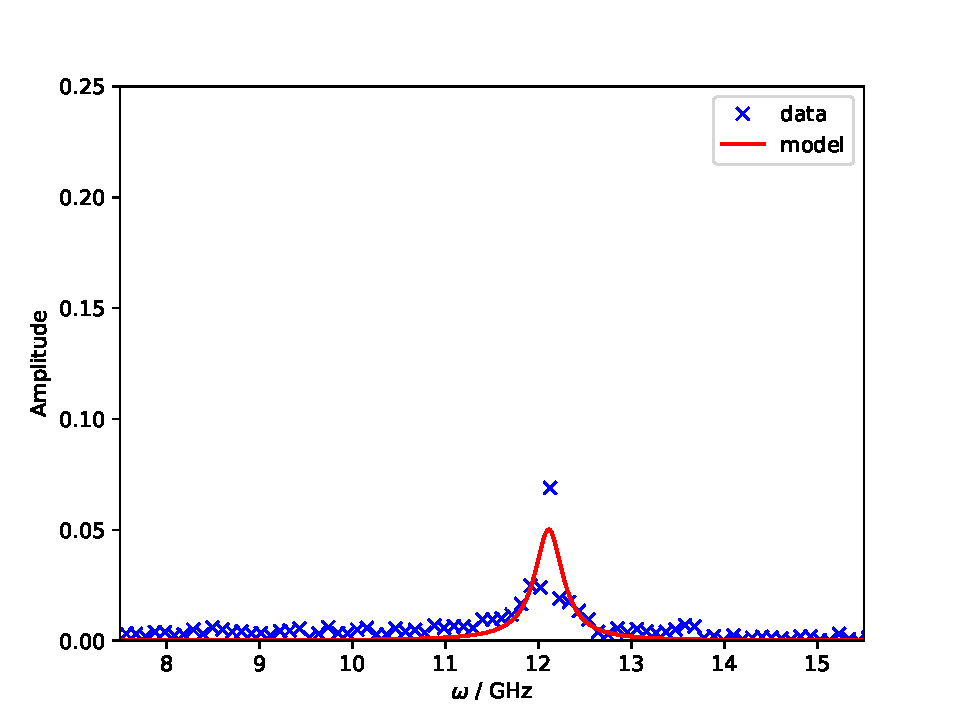
\includegraphics[width=\textwidth]{img/009_a000_b0_e245_G4_90fft.pdf}
 	\caption{Frequenzsprektrum für das 23\,nm tiefen Gitter unter einem Polarisationswinkel von 90 Grad}
 	\label{abb:film}
\end{figure}

\begin{table}[h!]
 \centering
\begin{tabular}{cc}
    Koeffizient & Wert \\
	\midrule
 	$\omega_0$ & 12,8 $\pm$ 0,4 \\
 	$\gamma$ & 0,9 $\pm$ 0,4 \\
\end{tabular}
\caption{Fit Ergebnisse für das Gitter mit 23\,nm tiefe unter einem Polarisationswinkel von 90 Grad}
\label{tab:fit}
\end{table}
\section{Verbesserung der Signalqualität mit Hilfe eines Tiefpasses}
\section{Diskussion}
Die errechneten g-Faktoren für Rb85 und Rb87 mit $g_{F,85} = 0,488 $\pm$ 0,005$ und
$g_{F,87} = 0,331 $\pm$ 0,002$ stimmen mit guter Genauigkeit mit den Theoriewerten von $\frac{1}{2}$ und $\frac{1}{3}$ überein.
Auch der Wert für die horizontal Komponente des Erdmagnetfeldes scheint unter Berücksichtigung der Größenordnung plausiebel zu sein.

Der Vergleich der Kernspins mit den Literaturwerten liefert ebenso eine zufriedenstellende Übereinstimmung.
Für Rb85 finden wir einen Kernspin von  I_{Rb,85} = $\frac{5}{2}$ und für Rb87 einen Kernspin von I_{Rb,87} = $\frac{3}{2}$, was im wesentlichen den Literaturwerten \cite{coreSpin} entspricht.

Das errechnete Isotopenverhältnis von r = 0,507 weicht signifikant vom Literaturwert von r = 0,386 \cit{isoVer} ab. Als mögliche Fehlerquelle
sei hier eine möglicherweise nicht komplett abgedunkelte Apparatur genannt. In diesem Fall hätte das einfallende Restlicht
einen Offset in der Amplitudentiefe der Resonanzen bewirkt.

Auch könnte die Speicherung als JPEG und die weitere Verarbeitung mit gimp einen Fehler begründen.

Die Abschätzung des quadratischen Zeemann-Effektes zeigt, das der quadratische Term bei den verwendeten Feldstärken drei Größenordnungen kleiner ist als der lineare Term. Daher kann der Einfluss des quadratischen Terms in guter Näherung vernachlässigt werden.

Der Theoriewerte des Verhältnisses $\frac{b_{87}}{b_{85}}$ ist 1,5 \cite{FP}. Somit weicht das Messergebnis von $\frac{b_{87}}{b_{85}} = 1,17 \pm 0,06$ um 22 Prozenpunkte vom Theoriewert ab.
Dieser Abweichung lässt sich damit begründen, dass das Zählen der Perioden nicht mit absoluter Genauigkeit möglich war.

\printbibliography


\end{document}
